\documentclass[fleqn, a4paper, 12pt]{article}
\usepackage{amsmath, amssymb, amsthm}
%\usepackage{gensymb}
\usepackage{commath}
\usepackage{xcolor}
\usepackage{siunitx}
\usepackage{tikz, pgfplots}
\usetikzlibrary{calc, hobby, patterns}
\usepackage{graphicx}
\usepackage{hyperref}
\usepackage{datetime}
\usepackage{ulem}
\usepackage{xfrac}
\usepackage{enumerate}
\setcounter{secnumdepth}{4}
\newcommand\numberthis{\addtocounter{equation}{1}\tag{\theequation}}

\newcommand{\AxisRotator}[1][rotate=0]{%
	\tikz [x=0.25cm,y=0.60cm,line width=.2ex,-stealth,#1] \draw (0,0) arc (-150:150:1 and 1);%
}

\theoremstyle{definition}
\newtheorem{example}{Example}
\newtheorem{definition}{Definition}

\theoremstyle{theorem}
\newtheorem{theorem}{Theorem}

\newenvironment{solution}
{\begin{proof}[Solution]\let\qed\relax}
	{\end{proof}}

\newcommand{\curl}{\mathrm{curl\,}}

%\renewcommand{\int_{min}^{max}}{\int\displaylimits_{min}^{max}}

%opening
\title{Lecture 11}
\author{Aakash Jog}
\date{\formatdate{2}{12}{2014}}

\begin{document}

\maketitle
%\setlength{\mathindent}{0pt}

\tableofcontents

\newpage
\section{Centre of Mass}

\begin{example}
	\begin{align*}
		\sigma = \dfrac{M_0}{\dfrac{1}{2} a b}
	\end{align*}
	\begin{tikzpicture}
		\coordinate (O) at (0,0);
		
		\def\xMIN{-1};
		\def\yMIN{-1};
		\def\xMAX{5};
		\def\yMAX{5};
		
		\def\a{3};
		\def\b{4};
	
		\coordinate (A) at (\a,0);
		\coordinate (B) at (0,\b);
	
	%	\draw [very thin, lightgray, step=1] (0,0,0) grid (4,4,4);
		\draw [<->, lightgray] (\xMIN,0) -- (\xMAX,0) node [right] {$x$};
		\draw [<->, lightgray] (0,\yMIN) -- (0,\yMAX) node [above] {$y$};
		
		\draw (O) -- node [midway, below] {$a$} (A) -- (B) -- node [midway, left] {$b$} cycle;
	\end{tikzpicture}\\
	Find the centre of mass of the triangle.
\end{example}

\begin{solution}
	\begin{align*}
		\dif m &= \left( -\dfrac{b}{a} x + b \right) \dif x \sigma\\
		\therefore x_{\text{COM}} &= \dfrac{\int x \dif m}{M_0}\\
		&= \dfrac{\int\limits_{0}^{a} x \left( -\dfrac{b}{a} x + b\right) \dif x \sigma}{M_0}\\
		&= \dfrac{\sigma \int\limits_{0}^{a} \left( -\dfrac{b}{a} x^2 + b x \right) \dif x }{M_0}\\
		&= \dfrac{M_0}{\dfrac{1}{2} a b M_0} \left( -\dfrac{b a^3}{3a} + \dfrac{b a^2}{2} \right)\\
		&= \dfrac{1}{3} a
	\end{align*}
\end{solution}

\begin{example}
	Find the COM of a solid cone.
\end{example}

\begin{solution}
	\begin{align*}
		\rho &= \dfrac{M_0}{\dfrac{1}{3} \pi R^2 H}\\
	\end{align*}
	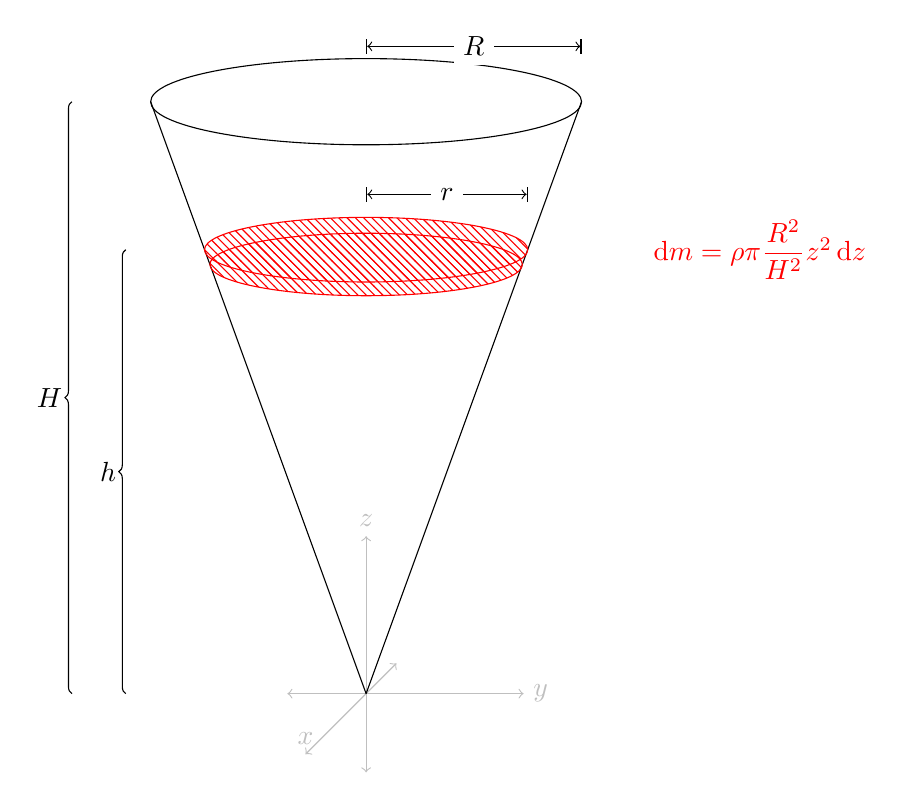
\begin{tikzpicture}
		%definition of origin
		\coordinate (O) at (0,0,0); 

		%definition of minimum and maximum values for axes
		\def\xMIN{-1};
		\def\yMIN{-1};
		\def\zMIN{-1};
		\def\xMAX{2};
		\def\yMAX{2};
		\def\zMAX{2};
		
		%axes
		\draw [<->, lightgray] (\xMIN,0,0) -- (\xMAX,0,0) node [right] {$y$}; 
		\draw [<->, lightgray] (0,\yMIN,0) -- (0,\yMAX,0) node [above] {$z$};
		\draw [<->, lightgray] (0,0,\zMIN) -- (0,0,\zMAX) node [above] {$x$};
		
		%definition of variables
		\def\L{8}; %diagonal length of cone
		\def\1_l{6}; %diagonal length of cone corresponding to upper edge of elemental disk
		\def\2_l{5.8}; %diagonal length of cone corresponding to lower edge of elemental disk
		\def\theta{20}; %half angle of cone
				
		%basic cone
		\draw (O) -- (90-\theta:\L);
		\draw (O) -- (90+\theta:\L);
		\draw (0, {\L*cos{\theta}}) circle [x radius = {\L*sin{\theta}}, y radius = {0.2*\L*sin{\theta}}];
		
		%dimensions of cone
		\draw [|<->|, yshift = 20] (0, {\L*cos{\theta}}) -- ++(0:\L*sin{\theta}) node [midway, fill=white] {$R$};
		\draw [decorate, decoration={brace}] (O) ++({-1-\L*sin{\theta}},0) -- ++(90:\L*cos{\theta}) node [left, midway] {$H$};
		
		%elemental disk
		\filldraw [red, pattern=north west lines, pattern color= red] (0, {\1_l*cos{\theta}}) circle [x radius = {\1_l*sin{\theta}}, y radius = {0.2*\1_l*sin{\theta}}] node [xshift=5cm] {$\dif m = \rho \pi \dfrac{R^2}{H^2} z^2 \dif z $};
		\filldraw [red, pattern=north west lines, pattern color= red] (0, {\2_l*cos{\theta}}) circle [x radius = {\2_l*sin{\theta}}, y radius = {0.2*\2_l*sin{\theta}}];
		
		%dimensions corresponding to elemental disk
		\draw [|<->|, yshift = 20] (0, {\1_l*cos{\theta}}) -- ++(0:\1_l*sin{\theta}) node [midway, fill=white] {$r$};
		\draw [decorate, decoration={brace}] (O) ++({-1-\1_l*sin{\theta}},0) -- ++(90:\1_l*cos{\theta}) node [left, midway] {$h$};
	\end{tikzpicture}
	\begin{align*}
		\dfrac{r}{R} &= \dfrac{z}{H}\\
		\therefore r &= \dfrac{R}{H} z
	\end{align*}
	\begin{align*}
		x_{\text{COM}} = y_{\text{COM}} &= 0\\
		z_{\text{COM}} &= \dfrac{\int\limits_{0}^{M_0} z \dif m}{M_0}\\
		&= \dfrac{\int\limits_{0}^{H} z \rho \pi \dfrac{R^2}{H^2} z^2 \dif z}{M_0}
	\end{align*}
\end{solution}

\section{Energy and Centre of Mass}

\begin{example}
	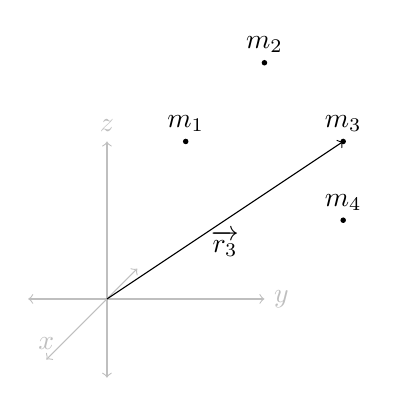
\begin{tikzpicture}
		%definition of origin
		\coordinate (O) at (0,0,0); 
		
		%definition of minimum and maximum values for axes
		\def\xMIN{-1};
		\def\yMIN{-1};
		\def\zMIN{-1};
		\def\xMAX{2};
		\def\yMAX{2};
		\def\zMAX{2};
		
		%axes
		\draw [<->, lightgray] (\xMIN,0,0) -- (\xMAX,0,0) node [right] {$y$}; 
		\draw [<->, lightgray] (0,\yMIN,0) -- (0,\yMAX,0) node [above] {$z$};
		\draw [<->, lightgray] (0,0,\zMIN) -- (0,0,\zMAX) node [above] {$x$};
		
		\coordinate (m1) at (1, 2);
		\coordinate (m2) at (2, 3);
		\coordinate (m3) at (3, 2);
		\coordinate (m4) at (3, 1);
		
		\fill (m1) circle [radius=1pt] node [above] {$m_1$};
		\fill (m2) circle [radius=1pt] node [above] {$m_2$};
		\fill (m3) circle [radius=1pt] node [above] {$m_3$};
		\fill (m4) circle [radius=1pt] node [above] {$m_4$};
		
		\draw [->] (O) -- (m3) node [midway, below] {$\overrightarrow{r_3}$};
	\end{tikzpicture}
\end{example}

\begin{solution}
	\begin{align*}
		\overrightarrow{r_k} &= \overrightarrow{r_{\text{COM}}} + \overrightarrow{r'_k}\\
		\therefore \overrightarrow{v_k} &= \overrightarrow{v_{\text{COM}}} + \overrightarrow{v'_k}
	\end{align*}
	\begin{align*}
		E_{\text{kinetic}} &= \sum \dfrac{1}{2} m_i (\dot{\overrightarrow{r_i}})^2\\
		&= \sum \dfrac{1}{2} m_i (\overrightarrow{v_i})^2\\
		&= \sum \dfrac{1}{2} m_i (\overrightarrow{v_{\text{COM}}} + \overrightarrow{v'_k})^2\\
		&= \sum \dfrac{1}{2} m_i (\overrightarrow{v_{\text{COM}}} + \overrightarrow{v'_k})\cdot(\overrightarrow{v_{\text{COM}}} + \overrightarrow{v'_k})\\
		&= \sum \dfrac{1}{2} m_i (v_{\text{COM}})^2 + \sum \dfrac{1}{2} m_i \overrightarrow{v_{\text{COM}}} \cdot \overrightarrow{v'_k} + \sum \dfrac{1}{2} m_i (v_{k})^2\\
		&= \dfrac{1}{2} \left(\sum m_i\right) (v_{\text{COM}})^2 + \overrightarrow{v_{\text{COM}}} \left(\sum m_i \overrightarrow{v_{k}}\right) + E'_{\text{kinetic}}\\
		&= \dfrac{1}{2} \left(\sum m_i\right) (v_{\text{COM}})^2 + 0 + E'_{\text{kinetic}}\\
		&= \dfrac{1}{2} M_{\text{total}} (v_{\text{COM}})^2 + E'_{\text{kinetic}}
	\end{align*}
\end{solution}

\begin{example}
	Find the maximum compression of the spring.\\
	\begin{tikzpicture}
		%definition of origin
		\coordinate (O) at (0,0,0); 
		
		%definition of minimum and maximum values for axes
		\def\xMIN{-1};
		\def\yMIN{-1};
		\def\zMIN{-1};
		\def\xMAX{2};
		\def\yMAX{2};
		\def\zMAX{2};
		
		\coordinate (A) at (-2,0);
		\coordinate (B) at (0,0);
		\coordinate (C) at (4,0);
		\coordinate (spring beginning) at (1, 0.5);
		\coordinate (spring end) at (4, 0.5);
		
		%axes
		\draw [<->, lightgray] (\xMIN,0,0) -- (\xMAX,0,0) node [below] {$x$};
		\draw [<->, lightgray] (0,\yMIN,0) -- (0,\yMAX,0) node [left] {$y$};

		\draw (-5, 0) -- (5,0);
		
		\draw (A) rectangle node {$m$} ++(1,1);
			\draw [->] (A) ++(0,1.5) -- ++(0:1) node [right] {$v_0$};
		
		\draw (B) rectangle node {$m$} ++(1,1);
		
		\draw [decorate, decoration={coil, segment length=5pt, aspect=0.7}] (spring beginning) -- (spring end);
		
		\draw (C) rectangle node {$m$} ++(1,1);

	\end{tikzpicture}
\end{example}

\begin{solution}
	As during the collision, mechanical energy is not conserved, COME cannot be applied to the system. However COLM can be applied  in the $x$ direction, as the net force is zero. \\
	\begin{tikzpicture}
		%definition of origin
		\coordinate (O) at (0,0,0); 
		
		%definition of minimum and maximum values for axes
		\def\xMIN{-1};
		\def\yMIN{-1};
		\def\zMIN{-1};
		\def\xMAX{2};
		\def\yMAX{2};
		\def\zMAX{2};
		
		\coordinate (A) at (-1,0);
		\coordinate (B) at (0,0);
		\coordinate (C) at (4,0);
		\coordinate (spring beginning) at (1, 0.5);
		\coordinate (spring end) at (4, 0.5);
		
		%axes
		\draw [<->, lightgray] (\xMIN,0,0) -- (\xMAX,0,0) node [below] {$x$};
		\draw [<->, lightgray] (0,\yMIN,0) -- (0,\yMAX,0) node [left] {$y$};
		
		\draw (-5, 0) -- (5,0);
		
		\draw (A) rectangle node {$m$} ++(1,1);
			\draw [->] (A) ++(0.5,1.5) -- ++(0:1) node [right] {$\dfrac{v_0}{2}$};
		
		\draw (B) rectangle node {$m$} ++(1,1);
		
		\draw [decorate, decoration={coil, segment length=5pt, aspect=0.7}] (spring beginning) -- (spring end);
		
		\draw (C) rectangle node {$m$} ++(1,1);
	\end{tikzpicture}\\
	\begin{align*}
		v_{\text{COM}} &= \dfrac{m v_0 + m(0) + m(0)}{3m}\\
		&= \dfrac{v_0}{3}\\
		p_{\text{total}} &= m v_0
	\end{align*}
	Consider the time of collision of the bodies to be $t = 0$.\\
	Therefore,
	\begin{align*}
		x_{\text{COM}}(t = 0) = \dfrac{l}{3}
	\end{align*}
	Therefore, in the COM frame of reference,\\
	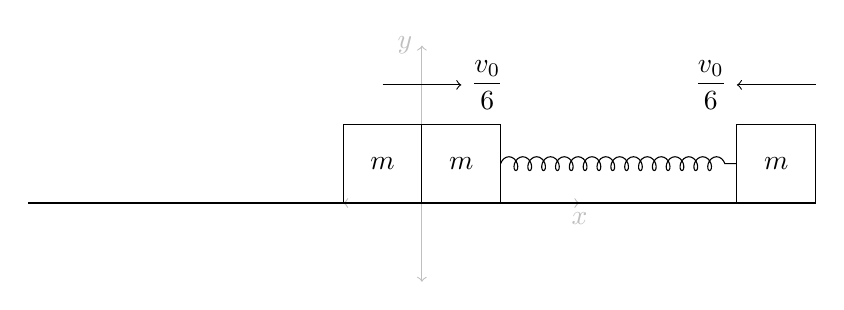
\begin{tikzpicture}
		%definition of origin
		\coordinate (O) at (0,0,0); 
		
		%definition of minimum and maximum values for axes
		\def\xMIN{-1};
		\def\yMIN{-1};
		\def\zMIN{-1};
		\def\xMAX{2};
		\def\yMAX{2};
		\def\zMAX{2};
		
		\coordinate (A) at (-1,0);
		\coordinate (B) at (0,0);
		\coordinate (C) at (4,0);
		\coordinate (spring beginning) at (1, 0.5);
		\coordinate (spring end) at (4, 0.5);
		
		%axes
		\draw [<->, lightgray] (\xMIN,0,0) -- (\xMAX,0,0) node [below] {$x$};
		\draw [<->, lightgray] (0,\yMIN,0) -- (0,\yMAX,0) node [left] {$y$};
		
		\draw (-5, 0) -- (5,0);
		
		\draw (A) rectangle node {$m$} ++(1,1);
			\draw [->] (A) ++(0.5,1.5) -- ++(0:1) node [right] {$\dfrac{v_0}{6}$};
		
		\draw (B) rectangle node {$m$} ++(1,1);
		
		\draw [decorate, decoration={coil, segment length=5pt, aspect=0.7}] (spring beginning) -- (spring end);
		
		\draw (C) rectangle node {$m$} ++(1,1);
					\draw [->] (C) ++(1,1.5) -- ++(180:1) node [left] {$\dfrac{v_0}{6}$};
	\end{tikzpicture}\\
	Therefore, 
	\begin{align*}
		E' &= \dfrac{1}{2} (2m) \left(\dfrac{v_0}{6}\right)^2 + \dfrac{1}{2} m \left(\dfrac{1}{3} v_0\right)^2\\
		&= \dfrac{3 m v_0^2}{36}\\
		&= \dfrac{1}{12} m v_0^2
	\end{align*}
	After the collision, we can apply COME to the system.\\
	Therefore,
	\begin{align*}
		\dfrac{1}{2} k x_{\text{max}}^2 &= \dfrac{1}{12} m v_0^2\\
		\therefore x_{\text{max}} &= \sqrt{\dfrac{m v_0^2}{6 k}}
	\end{align*}
\end{solution}

\end{document}